\subsection{DAC Power Amp} \label{subsec:DAC_Filter}
The system is to test impedance over a broad range of \SIQ{100}{\milli\ohm} to \SIQ{100}{\mega\ohm}, according to requirement §3 from section \ref{ch:SystemRequirements}. In order to excite impedances, especially in the range of \SIQ{10}{\ohm} and lower, a power amplifier is required. This amplifier must be capable of driving both reactive and passive devices. This is achieved by the use of controlled output impedance and the utilized range resistors used to measure the DUT current. 

The amplifier is designed as a class AB amplifier output stage and a high speed op-amp. The circuit used can be seen in figure \ref{fig_7_1_1_5_DAC_POWER_AMP}.

\begin{figure}[H]
    \centering
    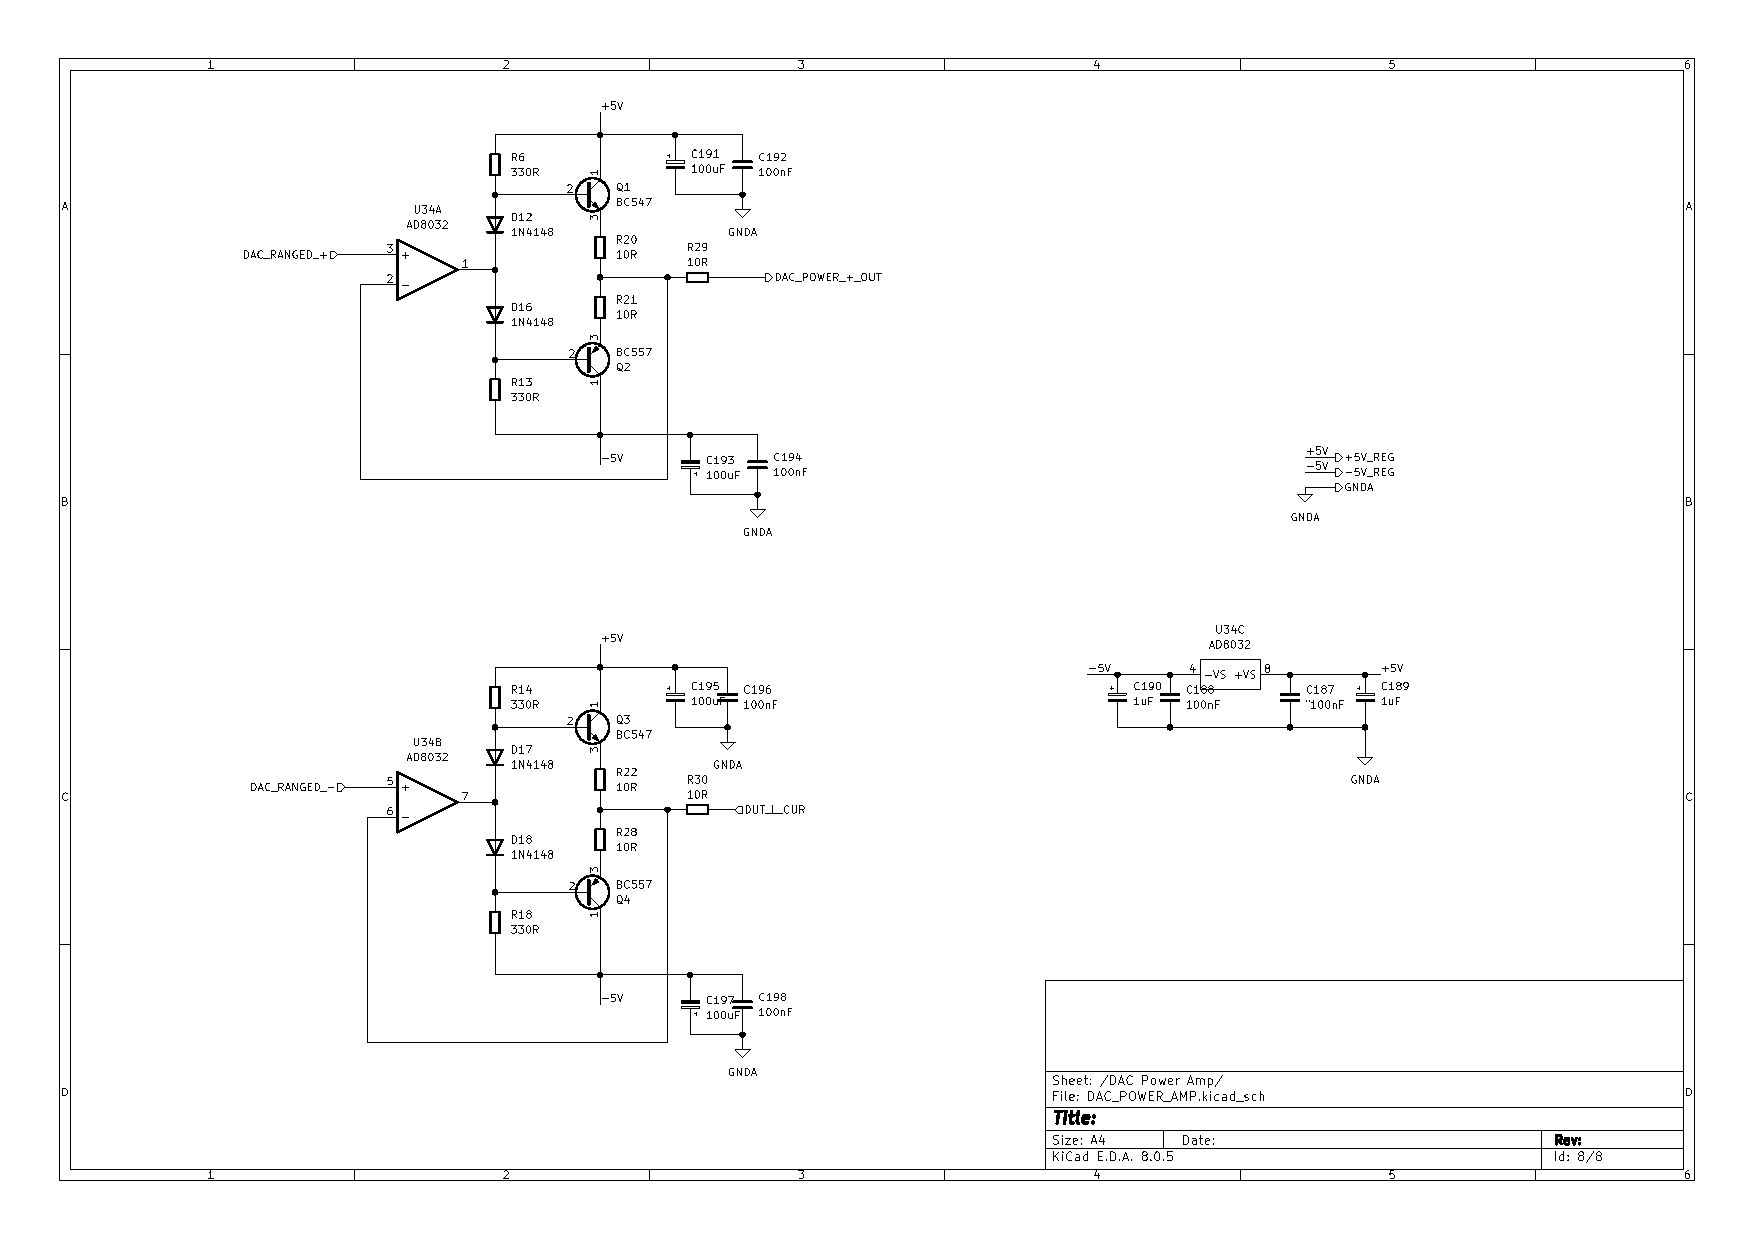
\includegraphics[clip, trim=150 320 440 40, width=0.9\textwidth]{Sections/7_SystemDesign/Figures/7_1_1_5_DAC Power Amp.pdf}
    \caption{DAC power amplifier circuit, positive side of the differential output.}
    \label{fig_7_1_1_5_DAC_POWER_AMP}
\end{figure}

About \SIQ{15}{\milli\ampere} of bias current for the output stage has been chosen. From BC547B and BC557 datasheets, \cite{BC547_datasheet} \cite{BC557_datasheet}, the base-emitter voltage can be found to be roughly \SIQ{730}{\milli\volt} at a collector current of \SIQ{15}{\milli\ampere}. This bias-current is set by the use of a simply diode. This adds some thermal stability, given they are thermally closely linked, as the temperature coefficient of a diode is negative, whilst positive for a transistor. The required DC current for a 1n4148 diode to have a voltage-drop of \SIQ{730}{\milli\volt} is estimated to \SIQ{12}{\mA}. The supply voltage is from a split supply of $\pm$ \SIQ{5}{\volt}, resulting in a total supply voltage of \SIQ{10}{\volt}. Assuming that the two biasing diodes, D12 and D16 in figure \ref{fig_7_1_1_5_DAC_POWER_AMP}, are matched the voltage across the biasing resistors R6 and R13 will be $10-2\cdot0.73 = $\SIQ{8.54}{\volt}. Combined series resistance of R6 and R13 can be estimated as $\frac{8.54 V}{0.012 A} = $ \SIQ{712}{\ohm}. Resistors of \SIQ{330}{\ohm} has been chosen, producing a biasing current of \SIQ{12.9}{\milli\ampere}.

To increase the input impedance and reduce output distortion of the amplifier, an op-amp is used with the output class AB stage in its feedback loop. The used op-amp is an \SIQ{80}{\mega\hertz} GBW op-amp, AD8032 \cite{AD8032_datasheet}. 

\subsubsection{Stability}
Driving reactive, especially capacitive loads as they ideally add \SIQ{-90}{\degree} phase shift, can pose a challenge to any feedback system, such as op-amps. The typical phase-margin of an op-amp is in the range of \SIQ{45}{\degree}. This will result in an unstable feedback system if the phase drops more than the phase margin of the used op-amp. This leads to the conclusion that most feedback systems will be unstable when driving any ideal capacitor.

A way to reduce the risk of instability, a zero can be introduced in the transfer function of the feedback path. This zero can remove the introduced \SIQ{-90}{\degree} phase of the capacitor. This can be realized simply be placing a resistor in series with the output of feedback system. This resistor should be placed outside of the feedback loop. The value of this resistor will depend upon the load capacitor.